\pagestyle{empty}
\tikzstyle{every picture}+=[remember picture]
\everymath{\displaystyle}

\begin{figure}[!ht]

\centering
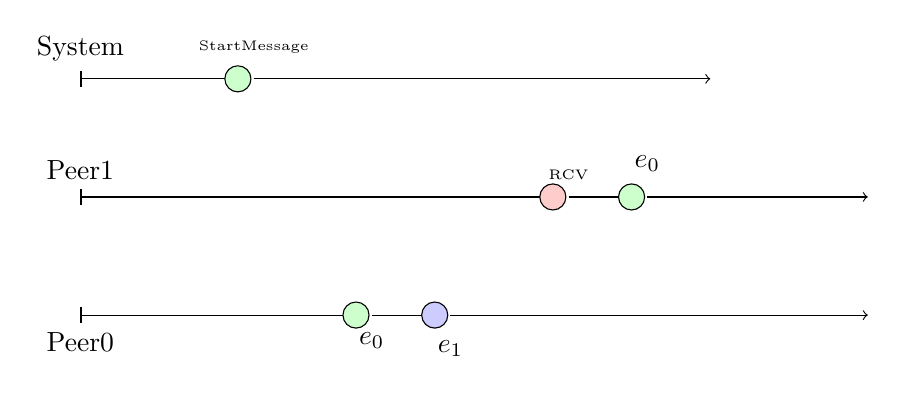
\begin{tikzpicture}

% PEER 1

\draw[|-] (0,0) node[below=1mm]{Peer0} -- (3.5,0) node{\tikz[baseline]{
	\node[fill=green!20,draw,circle] (e0){};
}
};
\draw[-] (3.7,0) node[below=1mm]{$e_0$} -- (4.5,0) node{\tikz[baseline]{
	\node[fill=blue!20,draw,circle] (e1){};
}
};
\draw[->] (4.7,0) node[below=2mm]{$e_1$} -- (10,0) node[below=1mm]{};

% PEER 0

\draw[|-] (0,1.5) node[above=1mm]{Peer1} -- (6,1.5) node{\tikz[baseline]{
	\node[fill=red!20,draw,circle] (f0){};
}
};
\draw[-] (6.2,1.5) node[above=1mm]{\tiny{RCV}} -- (7,1.5) node{\tikz[baseline]{
	\node[fill=green!20,draw,circle] (f1){};
}
};
\draw[->] (7.2,1.5) node[above=2mm]{$e_0$} -- (10,1.5) node[below=1mm]{};

% SYSTEM TIMELINE

\draw[|-] (0,3) node[above=1mm]{System} -- (2,3) node{\tikz[baseline]{
	\node[fill=green!20,draw,circle] (sm){};
}
};
\draw[->] (2.2,3) node[above=2mm]{\tiny{StartMessage}} -- (8,3) {};

\end{tikzpicture}

% Now it's time to draw some edges between the global nodes. Note that we
% have to apply the 'overlay' style.
\begin{tikzpicture}[overlay]
        \path[->] (sm) edge [out=-90, in=135] (e0);
        \path[->] (sm) edge [out=-45, in=135] (f1);
        \path[->] (e1) edge [out=45, in=-135] (f0);
\end{tikzpicture}

  \caption{An overcomed issue in our asyncronous simulation.}
\end{figure}
